\documentclass{article}\usepackage{amsmath,amssymb,amsthm,tikz,tkz-graph,color,chngpage,soul,hyperref,csquotes,graphicx,floatrow}\newcommand*{\QEDB}{\hfill\ensuremath{\square}}\newtheorem*{prop}{Proposition}\renewcommand{\theenumi}{\alph{enumi}}\usepackage[shortlabels]{enumitem}\usepackage[nobreak=true]{mdframed}\usetikzlibrary{matrix,calc}\MakeOuterQuote{"}\usepackage[margin=0.75in]{geometry} \newtheorem{theorem}{Theorem}

\title{EE16A - Lecture 12 Notes}
\author{Name: Felix Su$\quad$SID: 25794773}
\date{Spring 2016$\quad$GSI: Ena Hariyoshi}
\begin{document}
\maketitle

%%%% Topic %%%%
\subsection*{Power}
%%%% Notes %%%%
\begin{itemize}
\item Energy disappated over time: $P = \frac{Energy}{Time}$
\end{itemize}
\begin{mdframed}
\textbf{Power Equations:}\\
\begin{equation}P = VI = I^2R=\frac{V^2}{R}\end{equation}
\end{mdframed}

%%%% Topic %%%%
\subsection*{Thevenin Equivalence}
%%%% Notes %%%%
\begin{center}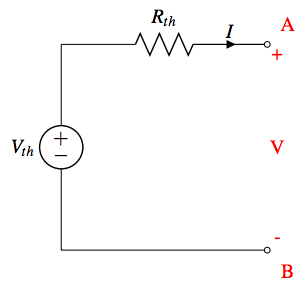
\includegraphics{thev}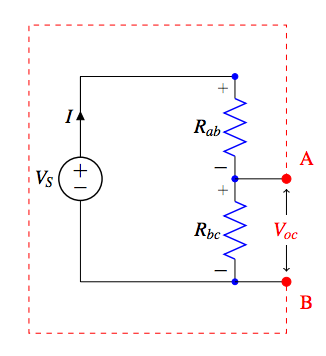
\includegraphics{th_voc}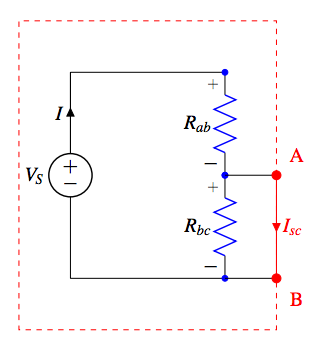
\includegraphics{th_isc}\end{center}
\begin{itemize}
\item Open Circuit: Find voltage drop between two nodes in complete  (normal) circuit ($V_{oc}$). No current is flowing (no voltage drop over resistor).
\item Short Circuit: Find current between two nodes, skip all voltage drops/resistors/subcircuits between them ($I_{sc}$)
\end{itemize}
\begin{mdframed}
\textbf{Thevenin Equations:}\\
\begin{equation}V_{th} = V_{oc}\end{equation}
\begin{equation}R_{th} = \frac{V_{th}}{I_{sc}}\end{equation}
\end{mdframed}

%%%% Topic %%%%
\subsection*{Norton Equivalence}
%%%% Notes %%%%
\begin{center}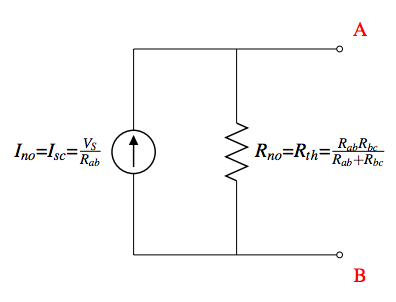
\includegraphics{norton}\end{center}
\begin{itemize}
\item Open Circuit:  Find voltage drop between two nodes in complete (normal) circuit $V_{oc} = I_{no}\cdot R_{no}$
\item Short Circuit: Find current between two nodes, skip all voltage drops/resistors/subcircuits between them ($I_{sc}$)
\end{itemize}
\begin{mdframed}
\textbf{Norton Equations:}\\
\begin{equation}I_{no}=I_{sc}=\frac{V_{S}}{R_{ab}}\end{equation}
\begin{equation}R_{no}=\frac{V_{oc}}{I_{no}} = \frac{R_{ab}R_{bc}}{R_{ab}+R_{bc}}=R_{th}=\frac{V_{th}}{I_{th}}\end{equation}
\end{mdframed}

\begin{mdframed}
\textbf{Thevenin/Norton Summary:}
\begin{itemize}
    \item Thevenin/Norton circuits have the same relationship between Voltage, $V$, in the circuit and the Current, $I$, coming out of it as the original circuits do
    \item They do not say anything about inside the actual circuit
    \item Ex. Power consumed by original circuit does not equal the power consumed by the T/N circuit (Power is non-linear)
\end{itemize}
\end{mdframed}

%%%% Topic %%%%
\subsection*{Superposition}
%%%% Notes %%%%
\begin{center}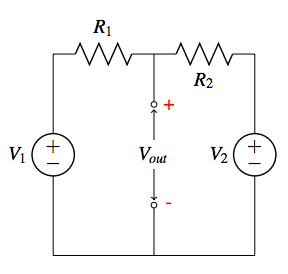
\includegraphics{spf}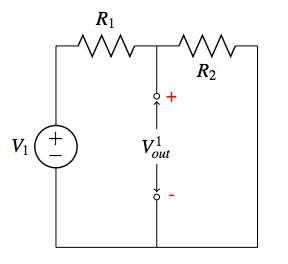
\includegraphics{sp1}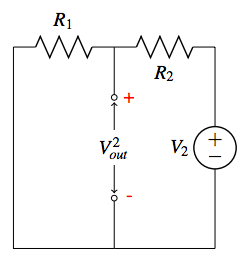
\includegraphics{sp2}\end{center}
\begin{enumerate}[1.]
    \item For each source ($V_{src}$, or $I_{src}$) $k$:
    \begin{enumerate}[a.]
        \item Set all other sources to 0
        \begin{itemize}
            \item $V_{src}$ to short circuit (no voltage drop/increase)
            \item $I_{src}$ to open circuit (no current)
        \end{itemize}
        \item Compute $V_{out}$ due to source $k$
    \end{enumerate}
    \item Sum up all $V_{out_k}$'s for all $k$ sources
\end{enumerate}

\end{document}